\documentclass[12pt]{article}
\usepackage[utf8]{inputenc}
\usepackage{float}
\usepackage{amsmath}

\usepackage[hmargin=3cm,vmargin=6.0cm]{geometry}
%\topmargin=0cm
\topmargin=-2cm
\addtolength{\textheight}{6.5cm}
\addtolength{\textwidth}{2.0cm}
%\setlength{\leftmargin}{-5cm}
\setlength{\oddsidemargin}{0.0cm}
\setlength{\evensidemargin}{0.0cm}

%misc libraries goes here
\usepackage[edges]{forest}
\usepackage{tcolorbox}
\usepackage{amsthm}
\usepackage{color, colortbl}
\usepackage{tikz}

\newtcolorbox{mybox}[3][]
{
  colframe = #2!25,
  colback  = #2!10,
  coltitle = #2!20!black,  
  title    = {#3},
  #1,
}

\newenvironment{explanation}[1][\unskip]{\begin{mybox}{red}{\textbf{Explanation} \textit{#1}}}{\end{mybox}}
\newenvironment{theorem}[1][\unskip]{\begin{mybox}{blue}{\textbf{Theorem} \textit{#1}}}{\end{mybox}}


\begin{document}

\section*{Student Information } 
%Write your full name and id number between the colon and newline
%Put one empty space character after colon and before newline
Full Name :  Burak Metehan Tunçel \\
Id Number :  2468726 \\


% Write your answers below the section tags
\section*{Answer 1}

I choose the Prim's algorithm to construct minimum spanning tree.

\subsection*{Answer of a}

\begin{table}[h!]
    \centering
    \begin{tabular}{| p{2cm} | p{2cm} | p{2cm}|}
        \hline
        \rowcolor{orange}
        Choice & Edge & Cost\\
        \hline
        \rowcolor{gray}
        1 & \{e,f\} & 1\\
        2 & \{e,h\} & 2\\
        \rowcolor{gray}
        3 & \{h,g\} & 2\\
        4 & \{c,f\} & 3\\
        \rowcolor{gray}
        5 & \{d,g\} & 3\\
        6 & \{a,d\} & 2\\
        \rowcolor{gray}
        7 & \{b,d\} & 3\\
        8 & \{h,i\} & 4\\
        \hline
    \end{tabular}
    \caption{The order in which the edges are added to the tree.}
    \label{tab:my_label}
\end{table}

\subsection*{Answer of b}

\begin{figure}[H]
	\centering
	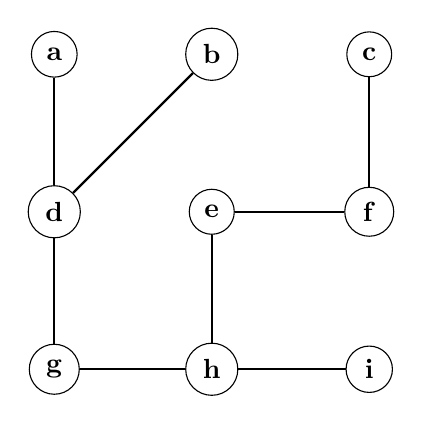
\begin{tikzpicture}
	
	\node[shape=circle,draw=black] (a) at (-2, 2)   {\textbf{a}};
	\node[shape=circle,draw=black] (b) at (0, 2)    {\textbf{b}};
	\node[shape=circle,draw=black] (c) at (2, 2)    {\textbf{c}};
	\node[shape=circle,draw=black] (d) at (-2, 0)   {\textbf{d}};
	\node[shape=circle,draw=black] (e) at (0, 0)    {\textbf{e}};
	\node[shape=circle,draw=black] (f) at (2, 0)    {\textbf{f}};
	\node[shape=circle,draw=black] (g) at (-2, -2)  {\textbf{g}};
	\node[shape=circle,draw=black] (h) at (0, -2)   {\textbf{h}};
	\node[shape=circle,draw=black] (i) at (2, -2)   {\textbf{i}};
	
	\path[-, thick] (e) edge (f);
	\path[-, thick] (e) edge (h);
	\path[-, thick] (h) edge (g);
	\path[-, thick] (c) edge (f);
	\path[-, thick] (d) edge (g);
	\path[-, thick] (a) edge (d);
	\path[-, thick] (b) edge (d);
	\path[-, thick] (h) edge (i);
	
	\end{tikzpicture} 
	\caption{The minimum spanning tree of the Graph $G$ in Figure 1.}
	\label{tab:my_label}
\end{figure}
The more common tree representation is the following
\begin{center}
\begin{forest}
for tree=
{
    grow=south,
    circle, draw, minimum size=1cm, inner sep=0.5cm,
    s sep=1cm
}
[\textbf{e}
    [\textbf{h}
        [\textbf{g}
            [\textbf{d}
                [\textbf{a}
                ]
                [\textbf{b}
                ]
            ]
        ]
        [\textbf{i}
        ]
    ]
    [\textbf{f}
        [\textbf{c}
        ]
    ]
]
\end{forest}
\end{center}

\subsection*{Answer of c}

The minimum spanning tree (MST), which is found the part b, is unique for the graph $G$ in Figure 1. However, in general, there is not absolute one MST for any connected edge-weighted undirected graph. That is, there can be more than 1 MST for a connected edge-weighted undirected graph.

As an example, there can be another MST if the edge (b,c) has weight 3 in graph $G$ in Figure 1. When it happens, b can also be connected from c instead of d.

\subsection*{Answer of d}

There are two mainly used algorithms to construct minimum spanning tree (MST), namely Prim's algorithm and Kruskal's algorithm. 

\noindent Both algorithm starts by choosing the minimum-weight/smallest-weight edge of the graph. If there is only one, unique, minimum-weight/smallest-weight edge, this edge has to be chosen by both algorithm at start. Therefore, this edge has to be included in the MST if there is a MST.


\newpage
\section*{Answer 2}

\noindent $G$ and $H$ are \textit{isomorphic}. $G$ and $H$ have the same number of vertices, number of edges, and number of vertices of each degree.

\begin{itemize}
    \item Both $G$ and $H$ have \underline{6} vertices and \underline{8} edges.
    \item Both have \underline{3} vertices of degree \underline{2}, \underline{2} vertices of degree \underline{3}, and \underline{1} vertex of degree \underline{4}.
\end{itemize}
Since $G$ and $H$ agree with respect to these invariants, it is reasonable to try to find an \textit{isomorphism} $f$.\\

\noindent The following one-to-one correspondence between $G$ and $H$ is the our \textit{isomorphism} $f$.

\begin{itemize}
    \item $f(a) = m$
    \item $f(b) = q$
    \item $f(c) = p$
    \item $f(d) = r$
    \item $f(e) = n$
    \item $f(f) = o$
\end{itemize}
So, $G$ and $H$ are \textit{isomorphic}.


\newpage
\section*{Answer 3}

\subsection*{Answer of a}

\begin{itemize}
    \item \textbf{Number of vertices:} 7
    \item \textbf{Number of edges:} 6
    \item \textbf{Height of $T$:} 3
\end{itemize}

\subsection*{Answer of b}

\begin{itemize}
    \item \textbf{Postorder:} (q:13), (s:19), (u:23), (v:58), (t:43), (r:24), (p:17)
    \item \textbf{Inorder:} (q:13), (p:17), (s:19), (r:24), (u:23), (t:43), (v:58)
    \item \textbf{Preorder:} (p:17), (q:13), (r:24), (s:19), (t:43), (u:23), (v:58)
\end{itemize}

\subsection*{Answer of c}

$T$ is \textit{a full binary tree}.

\begin{explanation}[Full Binary Tree]
A full binary tree is a tree in which every node other than the leaves has two children.\\

In other words, a full binary tree is a tree which every node has 0 or 2 children.
\end{explanation}

\noindent Since the every node of the $T$ has zero or two children, it can be told that $T$ is \textit{a full binary tree}.

\subsection*{Answer of d}

$T$ is \textit{not a complete binary tree}.

\begin{explanation}[Complete Binary Tree]
A complete binary tree is a binary tree in which every level, except possibly the last, is completely filled, and all nodes are as far left as possible.\\

In other words, a complete binary tree is a tree which all the levels are completely filled except possibly the last level and the last level has all keys as left as possible.
\end{explanation}

\noindent In $T$, the level 2 is not fully completed and the vertices in the last level are located in right instead of left.\\

\noindent Since $T$ does not satisfy the above explanation, it can be told that $T$ is \textit{not a complete binary tree}.

\subsection*{Answer of e}

$T$ is \textit{not a balanced binary tree}.

\begin{explanation}
If the subtrees at each vertex contain paths of approximately the same length, it can be told that the tree is balanced.\\

In other words, a balanced binary tree is a binary tree in which the height of the left and right subtree of any node differ by not more than 1 (0 or 1).
\end{explanation}

\noindent In $T$, the height of the left subtree of (p:17) is 0 whereas the height of the right subtree of (p:17) is 2. This indicates that it is not balanced.\\

\noindent Since $T$ does not satisfy the above explanation, it can be told that $T$ is \textit{not a complete binary tree}.

\subsection*{Answer of f}

$T$ is \textit{not a binary search tree}.

\begin{explanation}
A binary search tree is a rooted binary tree whose internal nodes each store a key greater than all the keys in the node’s left subtree and less than those in its right subtree.
\end{explanation}

\noindent In $T$, the right subtree of the (r:24) includes (u:23) whose key is 23. 23 is less than 24 ($23 \leq 24$); therefore, (u:23) should be located in the left subtree of (r:24) if $T$ is a binary search tree.\\

\noindent Since $T$ does not satisfy the above explanaiton, it can be told that $T$ is not \textit{not a binary search tree}.

\subsection*{Answer of g}

The answer is \textbf{11} according to following theorem.

\begin{theorem}[The minimum number of the nodes for a full binary tree with height $\lambda$]
The minimum number of the nodes for a full binary tree with height $\lambda$ is $2\lambda+1$
\end{theorem}

\begin{proof}
We can use induction to prove the above theorem.\\

\noindent \textbf{Basis Step:} If the height is 0 ($\lambda = 0$), there should be 1 node ($2 \times 0 + 1 = 1$). There will be only root node.

\noindent \textbf{Inductive Step:} Assume that the minimum number of nodes when height is $k$ ($\lambda = k$) is $2k+1$ is $N$.

When we add 1 node to the a leaf located at the deepest position (has the maximum height and the level count), the height will increase 1 and become $k+1$. To maintain a full binary tree, it will be necessary to add another node. In other words, the new level will need at least two more nodes. So, the number of nodes will be $N+2$.

Then, by our induction hypothesis $N + 2 = (2k + 1) + 2 = 2(k + 1) + 1$, which is what we wanted.\\
\end{proof}

\noindent In other words, basically, to achieve the full binary tree, there should be at least 2 nodes at each level except level 0 where root is located. So, for height 5, there should be 5 levels, each of which contains 2 nodes, and 1 root. $5 \times 2 + 1 = 11$.\\

One of the example full binary trees with height 5 and have the minimum number of the nodes is given below.

\begin{center}
\begin{forest}
for tree=
{
    grow=south,
    circle, draw, minimum size=1.5cm, inner sep=0.5cm,
    s sep=10mm
}
[1
    [2
        [4
            [6
                [8
                    [10
                    ]
                    [11
                    ]
                ]
                [9
                ]
            ]
            [7
            ]
        ]
        [5
        ]
    ]
    [3
    ]
]
\end{forest}
\end{center}


\end{document}